\documentclass[conference]{assets/latex/IEEEtran}
\IEEEoverridecommandlockouts

\usepackage{amsmath,amssymb,amsfonts}
\usepackage{graphicx}
\usepackage{textcomp}
\usepackage{xcolor}
\usepackage[backend=biber,style=numeric]{biblatex}
\addbibresource{assets/latex/report.bib}

\graphicspath{{assets/latex/}}

\begin{document}

\title{CS6524 Computer Vision Lab 3:\\ Structure from Motion}

\author{\IEEEauthorblockN{T\'{o}la Bowen MacCurt\'{a}in}
\IEEEauthorblockA{Student ID 23383372\\
University of Limerick}
\and
\IEEEauthorblockN{Naem Haq}
\IEEEauthorblockA{Student ID 23379243\\
University of Limerick}
}

\maketitle

\begin{abstract}
We reconstructed a vinyl figurine from two 12\,s phone videos: one where the camera orbits the
object (\textit{a}) and one where the camera is fixed and the object spins on a plate (\textit{b}).
The pipeline tracks KLT features verified against the essential matrix, localises each frame by PnP
against a growing map, refines it with windowed and global bundle adjustment, and fuses dense
optical-flow triangulations on a voxel grid. Across the twelve sensitivity runs the bundle-adjustment
error stayed between 0.34 and 0.65\,px, even in runs that recovered only 41$^\circ$ of the
360$^\circ$ rotation, so reprojection error alone did not tell good reconstructions from bad ones.
Removing lens distortion was decisive for video \textit{b} but not for \textit{a}, which we trace
to the limited image area covered by our Lab~2 calibration.
\end{abstract}

\section{Methodology}

\subsection{Capture and calibration}
Both videos were recorded on the same phone at $1080\times1920$ and downscaled to $360\times640$ at
10\,fps, giving 120 frames each (2.0\,MB and 0.8\,MB). In \textit{a} the figurine stands on a
sheet of paper on carpet; in \textit{b} it stands on a white plate that is turned by hand.
The intrinsics come from our Lab~2 calibration (24 frames, 0.209\,px mean reprojection error).
Since the videos were resized by $s=1/3$, we scaled the focal lengths by $s$ and the principal point
with the pixel-centre convention $c' = (c+0.5)s-0.5$, giving $f_x=587.55$, $f_y=586.91$,
$c_x=186.42$, $c_y=317.42$. The distortion coefficients $D$ are defined on normalised coordinates
and were kept unchanged ($k_1=0.169$, $k_2=-0.464$, $k_3=-3.483$). One caveat carried over from
Lab~2: the board only covered rows 432--997 of 1920 (rows 144--332 here), so $D$ is extrapolated
outside that band. Frames are undistorted with the same $K$, and a validity mask removes the black
wedges that undistortion leaves at the borders; their corners otherwise appear at the same pixel in
every frame and produce fake static matches.

\subsection{Keypoint selection (step 2)}
We compared SIFT and ORB (ratio test 0.75/0.8, one-to-one matching) with KLT
tracking~\cite{lucas1981} of Shi--Tomasi corners~\cite{shi1994} (at most 2000 corners, 7\,px apart,
$21\times21$ window, 3 pyramid levels, forward--backward error below 1\,px, new corners detected in
every frame). SURF is not available in the course image. Every consecutive match must be an inlier
of the essential matrix (RANSAC, 1\,px). Fig.~\ref{fig:tracks} shows how many tracks survive at
least $L$ frames. KLT keeps 293 (\textit{a}) and 419 (\textit{b}) tracks of 20 frames or more,
against 1 and 19 for SIFT and 13 and 34 for ORB: the descriptor methods re-detect in every frame,
so a single missed detection ends a track. We therefore used KLT for both videos.

In \textit{b} only the figurine moves rigidly with respect to the camera. Without a mask, only 35\%
of the verified KLT points lay on the figurine, and the longest track (all 120 frames) was a static
background point; people moving in the background and the hand turning the plate add further
outliers. We segment the figurine by colour (hue 27--45 in OpenCV HSV; its body is at 30--34, and
the lower bound excludes a plywood cabinet at 22--26 that the first version of the mask latched onto
in \textit{a}), add dark pixels within 40\,px of the body for the ears, tail and feet, and take the
dilated convex hull. Video \textit{a} uses the full frame, since its whole scene is static.

\begin{figure}[t]
\centerline{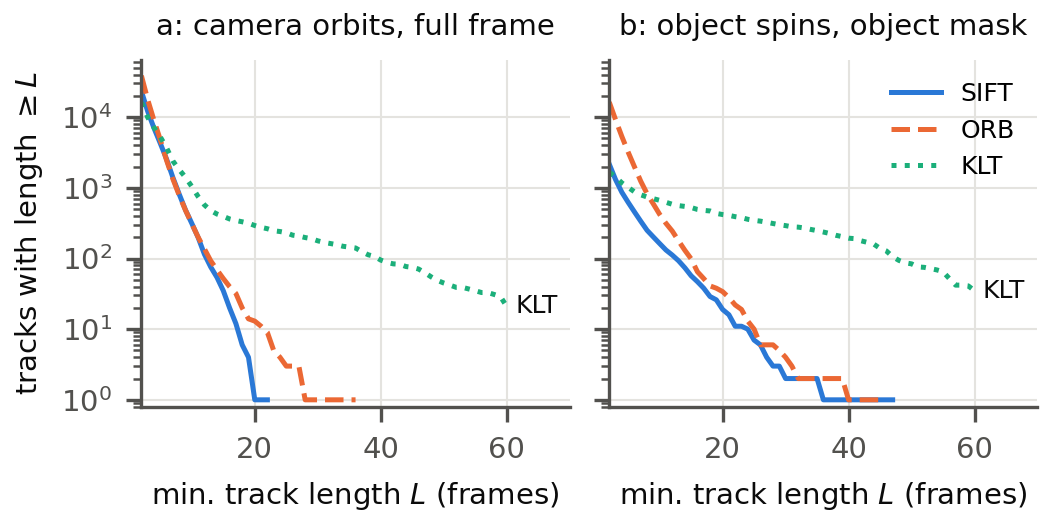
\includegraphics[width=\columnwidth]{step2_track_survival.png}}
\caption{Step~2: number of tracks that survive at least $L$ frames (log scale). Left: video
\textit{a}, full frame. Right: video \textit{b}, figurine mask.}
\label{fig:tracks}
\end{figure}

\subsection{Relative pose and two-view triangulation (steps 3--4)}
For every consecutive pair we estimate $E$ with the five-point algorithm~\cite{nister2004} inside
RANSAC and decompose it with a cheirality check into $R$ and a unit-length $t$~\cite{hartley2004}.
With frame $i$ as the origin, the inliers are triangulated and re-projected into both views; the mean
two-view reprojection error is 0.17--0.22\,px in every run. The reconstruction is initialised from
frames 0 and 4, because consecutive frames are only about 3$^\circ$ apart. Points are kept if they lie
in front of both cameras, re-project within 2\,px and have at least 1$^\circ$ of parallax.

\subsection{Extension to $N$ frames (step 5)}
Chaining the unit-length translations of consecutive pairs would give every pair its own scale.
Instead, each new frame is localised by PnP-RANSAC (2\,px, at least 8 inliers, Levenberg--Marquardt
refinement) against the 3D points already in the map, which keeps one scale. If PnP fails, we fall
back to the consecutive-pair $E$ and estimate its scale from the median depth ratio of shared points.
New tracks are triangulated between their first observation and the current frame. For the
correction we run bundle adjustment~\cite{triggs2000} on the last 10 frames every 5 frames (the
oldest two held fixed), followed by a global adjustment over all frames with frame 0 fixed
(\texttt{scipy} \texttt{least\_squares}, Huber loss at 1\,px, sparse Jacobian). Points with any
residual above 4\,px are then removed and the global adjustment is repeated.

Our first version failed in \textit{b}: the windowed error grew steadily from 0.44\,px at frame 10 to 5.9\,px at
frame 45, and PnP failed from frame 46 on. The cause was tracks that do not follow a fixed surface
point: specular highlights on the glossy figurine and points sliding along its silhouette as it
turns. We now split a track as soon as its 3D point re-projects more than 2\,px from the tracked
position: the earlier observations keep the point and the rest becomes a new track. With this change
\textit{b} reached the last frame without a PnP failure.

\subsection{Dense reconstruction (step 6)}
For frame pairs $(i, i+4)$ with $i$ stepping by 2 (58 pairs) we compute Farneb\"ack
flow~\cite{farneback2003} in both directions, keep pixels whose forward--backward error is below
0.5\,px, and triangulate every pixel of the region of interest (the figurine mask dilated by 40\,px in
\textit{a} and 12\,px in \textit{b}) with the bundle-adjusted poses. A point is kept if it
re-projects within 1.5\,px in both views and has at least 2$^\circ$ of parallax. To average across
frames, points are binned on a voxel grid whose size is 0.4\% of the cloud's extent; each voxel
stores the mean position and colour, and only voxels supported by at least three frame pairs are
kept. Requiring three pairs instead of two removed most of the floating points.

\subsection{Sensitivity protocol (step 7)}
We multiply $f_x$ and $f_y$ by 0.8, 1.0 and 1.2 and use the scaled $K$ everywhere, including
undistortion; $D$ is kept fixed, and the ``d'' runs skip undistortion. Since both videos cover a full
turn, we measure the trajectory against two loop properties. The swept rotation sums the per-frame
relative rotation vectors $\boldsymbol{\omega}_i$ projected on their mean axis $\hat{\mathbf{n}}$,
$\theta = \sum_i \boldsymbol{\omega}_i^{\top}\hat{\mathbf{n}}$ (ideally 360$^\circ$). The closure gap
is $\lVert C_{119}-C_0\rVert/\bar{r}$, where $C_i$ are the camera centres and $\bar{r}$ their mean
distance to the centroid (ideally 0). All numbers below come from the course Docker image
(OpenCV 5.0), the same image GitHub Actions uses.

\section{Results}

\begin{table}[t]
\caption{Results of the 12 runs (u: undistorted, d: distorted).}
\label{tab:results}
\centering\scriptsize\setlength{\tabcolsep}{3pt}
\begin{tabular}{lrrrrrr}
\hline
Run & Swept ($^\circ$) & Gap & BA (px) & PnP fail & Sparse & Dense \\
\hline
\texttt{a\_08u} & 258 & 2.21 & 0.56 & 3 & 3612 & 10511 \\
\texttt{a\_10u} & 279 & 2.10 & 0.50 & 3 & 6241 & 7410 \\
\texttt{a\_12u} & 285 & 1.83 & 0.49 & 4 & 9938 & 6128 \\
\texttt{a\_08d} & 192 & 3.00 & 0.52 & 6 & 7434 & 6128 \\
\texttt{a\_10d} & 300 & 1.14 & 0.34 & 1 & 10195 & 16864 \\
\texttt{a\_12d} & 354 & 0.29 & 0.36 & 0 & 12636 & 19263 \\
\texttt{b\_08u} & 300 & 1.13 & 0.54 & 0 & 2633 & 48855 \\
\texttt{b\_10u} & 287 & 1.47 & 0.54 & 0 & 2672 & 43657 \\
\texttt{b\_12u} & 122 & 4.11 & 0.58 & 2 & 2149 & 20030 \\
\texttt{b\_08d} & 58 & 3.38 & 0.64 & 10 & 1037 & 132 \\
\texttt{b\_10d} & 91 & 3.73 & 0.65 & 7 & 1211 & 1410 \\
\texttt{b\_12d} & 41 & 5.02 & 0.61 & 4 & 709 & 313 \\
\hline
\end{tabular}
\end{table}


\begin{figure}[t]
\centerline{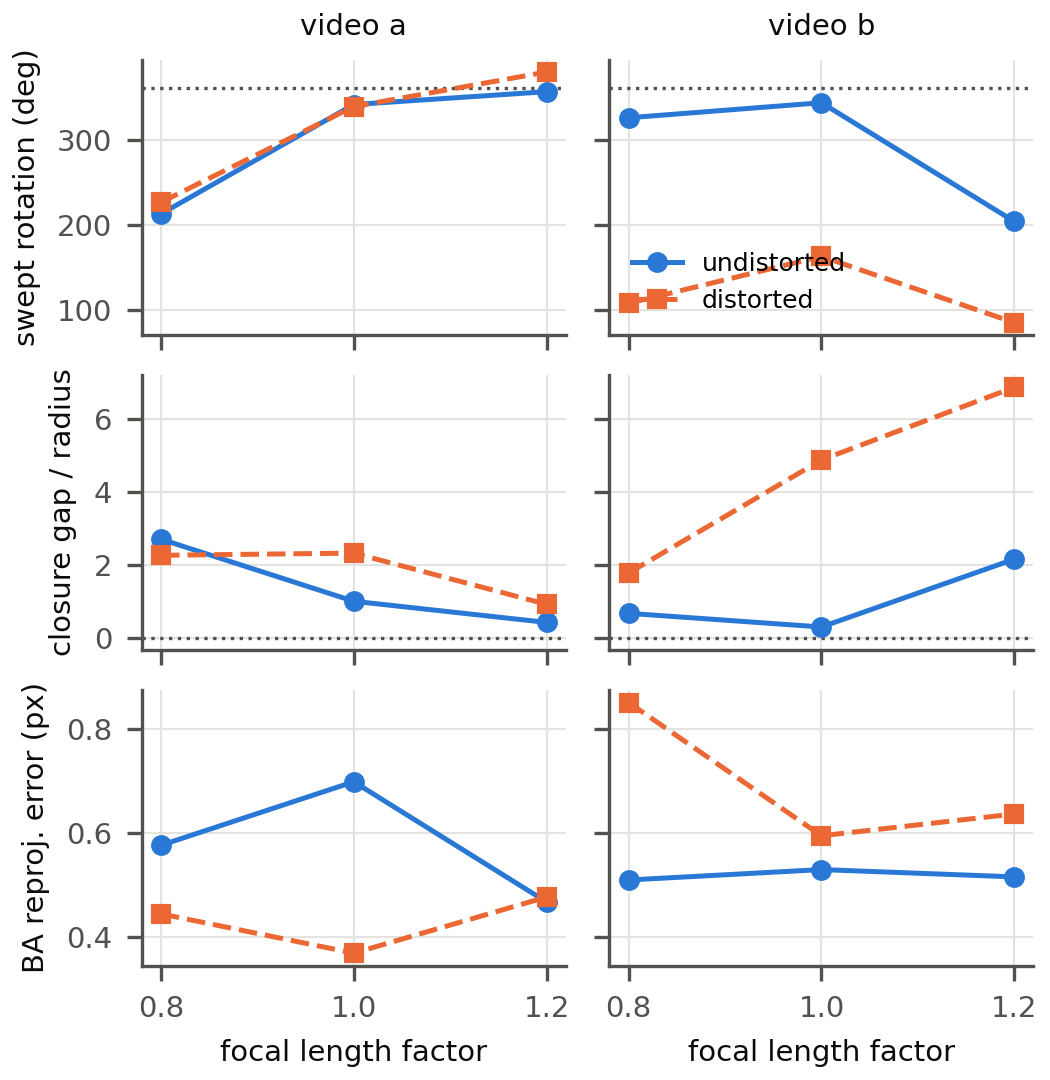
\includegraphics[width=\columnwidth]{step7_sensitivity.png}}
\caption{Step~7: swept rotation (ideal 360$^\circ$, dotted), closure gap (ideal 0) and final
bundle-adjustment error against the focal-length factor, with and without undistortion.}
\label{fig:sens}
\end{figure}

\begin{figure}[t]
\centerline{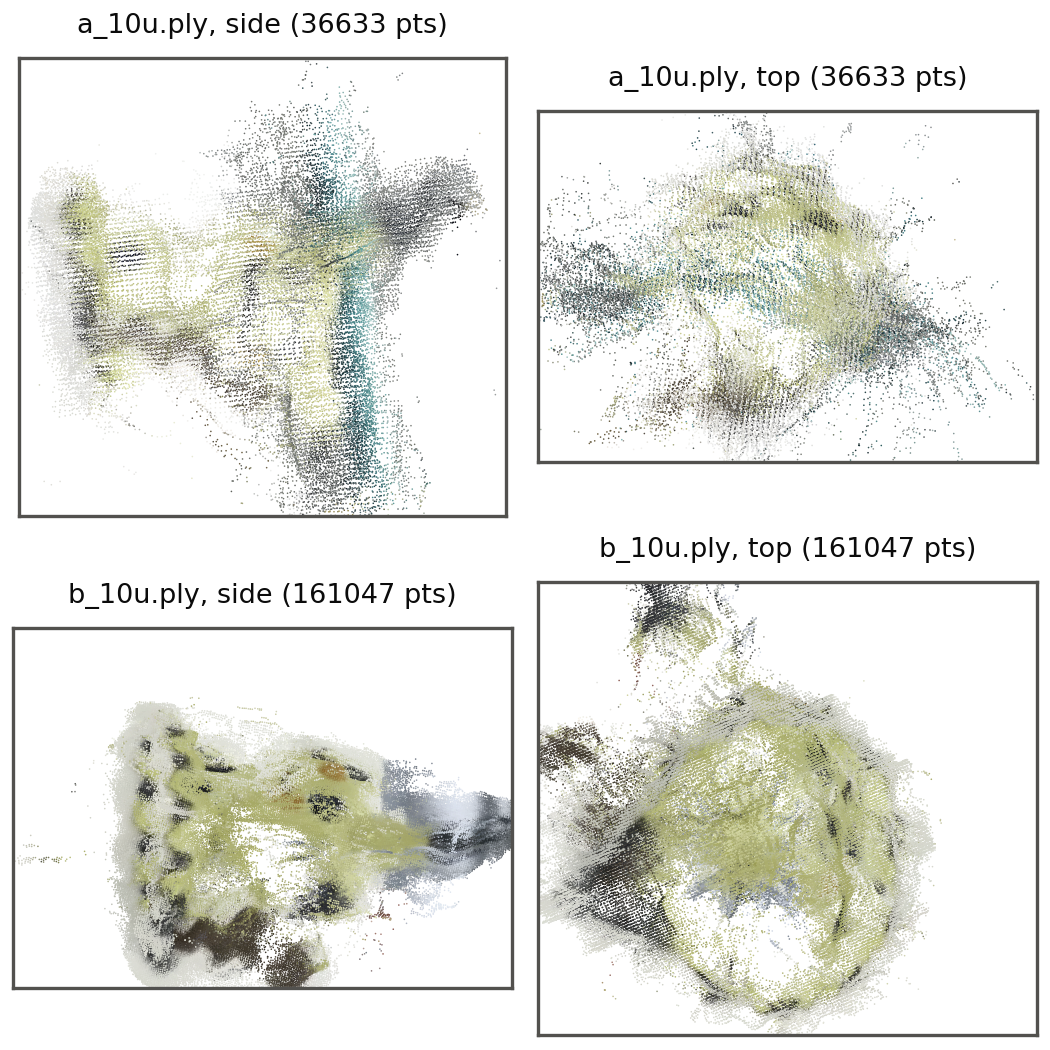
\includegraphics[width=\columnwidth]{step6_clouds.png}}
\caption{Dense clouds of the $f\times1.0$ undistorted runs, seen along their two main axes.}
\label{fig:clouds}
\end{figure}

Table~\ref{tab:results} and Fig.~\ref{fig:sens} summarise the twelve runs. The best trajectories
are \texttt{a\_12d} (354$^\circ$, gap 0.29, no PnP failures) and \texttt{b\_08u} (300$^\circ$, gap
1.13). For \textit{b}, the undistorted runs recover 122--300$^\circ$ with 0--2 PnP failures and
20k--49k dense points, while the distorted runs recover only 41--91$^\circ$ with 4--10 failures and
132--1410 dense points. For \textit{a} the pattern reverses: the distorted runs have more
essential-matrix inliers per pair (342--412 against 161--392) and contain the best run overall. The
dense clouds (Fig.~\ref{fig:clouds}) show the figurine's colours and dark feet in \textit{b}, but both
are blurred by overlapping surfaces from trajectory drift, and \textit{a} keeps few points.

\section{Discussion and failure analysis}

\textit{Reprojection error is not a quality measure here.} The final bundle-adjustment error is
0.34--0.65\,px in every run, including \texttt{b\_12d}, which recovered 41$^\circ$ of the
360$^\circ$ turn. A wrong $K$ or $D$ is absorbed into each pair's $E$ and into the adjusted poses;
it only shows as global inconsistency over the loop. The loop metrics were the only ones that
separated good runs from bad ones.

\textit{Distortion.} In \textit{b}, few points (709--2672) lie on a small object, so a systematic
1--2\,px error is the same size as our 2\,px PnP and splitting thresholds: tracks are cut, the map
runs dry, PnP fails, and every fallback injects a scale error. In \textit{a} the opposite happens,
and we believe the calibration explains it: most of the scene's texture is the carpet in the lower
half of the frame (in step~2 the median SIFT inlier was at row~500), outside the band 144--332 where
$D$ was estimated. Applying an extrapolated $D$ with $k_3=-3.48$ there seems to add error rather than
remove it.

\textit{Focal length.} To first order, a rotation $\Delta\theta$ moves image points by about
$f\Delta\theta$, so a factor of 0.8 should inflate the swept rotation towards 450$^\circ$ and 1.2
should shrink it towards 300$^\circ$. We do not see this: in \textit{a} the swept rotation and the
number of inliers both increase with $f$, and in \textit{b} the 1.2 run collapses. PnP failures and
drift dominate the trend more than the intrinsics do. The steady rise in inliers with $f$ in
\textit{a} could also mean our calibrated $f$ is too small for that recording (for example if the
phone crops the sensor for video stabilisation), but we did not test this.

\textit{Drift and loop closure.} No run closes the loop (gap $\geq$ 0.29). Around frames 94--107 of
\textit{a} the camera moved quickly and verified KLT links dropped from about 490 per pair to 37--143,
which caused the 3--6 PnP failures in four of the six \textit{a} runs. Each fallback changes the
scale; in our laptop runs this appeared in the dense cloud as a doubled, offset copy of the figurine. The 445--2863 track splits per
run show how often KLT follows highlights and silhouettes on a glossy object.

\textit{Reproducibility.} The same code on OpenCV 4.12 (our laptop) produced 343$^\circ$ and a gap
of 0.30 for \texttt{b\_10u}, against 287$^\circ$ and 1.47 in the course image. Small numerical
differences in tracking and RANSAC flip individual PnP results, so the pipeline sits close to a
failure threshold.

\textit{Improvements with more time.} (i) Close the loop by matching frame 0 to frame 119 with ORB and
adding those observations to the global adjustment; (ii) choose keyframe pairs by parallax instead of
fixed gaps, and relocalise a lost frame against older keyframes instead of falling back to $E$;
(iii) recalibrate with board views that cover the whole image; (iv) record \textit{a} with a slower
orbit or higher frame rate, and \textit{b} on a textured turntable with a matte object.

\printbibliography

\end{document}
